\documentclass[12pt]{article}
% --- Paquetes Necesarios ---
\usepackage[spanish]{babel}
\usepackage[utf8]{inputenc}
\usepackage{amsmath} 
\usepackage{amsfonts}
\usepackage{geometry}
\usepackage{graphicx}
\usepackage{float}
\usepackage{algorithm} 
\usepackage{algorithmic}
\usepackage{booktabs} 
\usepackage{hyperref}
\usepackage[plain,vlined]{algorithm2e}
\geometry{letterpaper, margin=1in}
\title{
    \includegraphics[width=0.6\textwidth]{logo udp.png} \\ 
    \vspace{1cm}
    \textbf{Algoritmos Exactos y Metaheurísticas: Tarea 1} 
}
\author{Dante Libiot , Claudio Alvial, Francisco Olmos \\ Profesor: Víctor Reyes \\ Ayudante: Diego Banda} 
\date{ 29 de marzo, 2026} 
\begin{document}
\maketitle
\newpage
\tableofcontents 
\newpage

% ============================================================
\section{Introducción} 
% ============================================================
Para abordar el problema de aterrizaje de aviones (Aircraft Landing Problem), se modeló el escenario como un Problema de Satisfacción de Restricciones (CSP) optimizado. La resolución se llevó a cabo mediante un algoritmo exacto basado en Backtracking (Búsqueda en Profundidad o DFS). El núcleo del algoritmo se encarga de asignar a cada avión $i$ una pista de aterrizaje $p$ y un tiempo específico $t$, con el objetivo de minimizar la función de penalización por aterrizar fuera del tiempo preferente ($P$). Para evitar la exploración exhaustiva de un espacio de búsqueda intratable cuya complejidad en el peor de los casos es $O((P \cdot T)^D)$ (donde $P$ es el número de pistas, $T$ la ventana de tiempo y $D$ la cantidad de aviones), el diseño incorpora un sistema de poda por cota superior (actualizando dinámicamente el mejor costo global) y técnicas de propagación de restricciones hacia el futuro.

% ============================================================
\section{Desarrollo}
% ============================================================

\subsection{Modelo del Problema} 
Definición formal del problema de optimización con restricciones para la programación y asignación de aterrizajes.

\subsubsection{Conjuntos}
\begin{itemize}
    \item $K$: Conjunto de aviones a programar, donde $k \in \{1, \dots, D\}$.
    \item $P$: Conjunto de pistas de aterrizaje disponibles.
\end{itemize}

\subsubsection{Parámetros}
\begin{itemize}
    \item $E_k$: Tiempo mínimo en el que el avión $k$ puede aterrizar.
    \item $L_k$: Tiempo máximo tolerado para el aterrizaje del avión $k$.
    \item $P_k$: Tiempo preferente de aterrizaje para el avión $k$.
    \item $C_k$: Costo de penalización si el avión $k$ aterriza antes de su tiempo preferente ($T_k < P_k$).
    \item $C'_k$: Costo de penalización si el avión $k$ aterriza después de su tiempo preferente ($T_k > P_k$).
    \item $\tau_{ij}$: Tiempo mínimo de separación requerido por seguridad entre el avión $i$ y el avión $j$.
\end{itemize}

\subsubsection{Variables de Decisión}
\begin{itemize}
    \item $T_k$: Variable entera que representa el tiempo exacto de aterrizaje asignado al avión $k$.
    \item $X_{kp}$: Variable binaria que toma el valor 1 si el avión $k$ es asignado a la pista $p$, y 0 en caso contrario.
    \item $y_k$: Variable binaria indicadora de retraso; toma el valor 1 si el avión excede su tiempo preferente, 0 en otro caso.
    \item $n_k$: Variable binaria indicadora de adelanto; toma el valor 1 si el avión llega antes de su tiempo preferente, 0 en otro caso.
\end{itemize}

\subsubsection{Función Objetivo}
El objetivo fundamental del modelo es minimizar el costo total asociado a las penalizaciones económicas por aterrizar de forma temprana o tardía:
$$ \min Z = \sum_{k=1}^{D} \left( (T_k - P_k) \cdot y_k \cdot C_k + (P_k - T_k) \cdot n_k \cdot C'_k \right) $$

\subsubsection{Restricciones}
\begin{itemize}
    \item \textbf{Ventanas de tiempo de seguridad:} El tiempo asignado debe estar estrictamente dentro de los límites operativos del avión:
    $$ T_k \ge E_k, \quad \forall k \in K $$
    $$ T_k \le L_k, \quad \forall k \in K $$
    
    \item \textbf{Asignación única de pista:} Todo avión debe ser asignado a exactamente una pista de aterrizaje:
    $$ \sum_{p \in P} X_{kp} = 1, \quad \forall k \in K $$
    
    \item \textbf{Separación mínima por estela turbulenta:} Si el avión $j$ es programado para aterrizar después del avión $i$ ($T_j > T_i$), se debe garantizar la distancia de tiempo obligatoria:
    $$ T_j \ge T_i + \tau_{ij} $$
    
    \item \textbf{Linealización de las penalidades:} Para acotar la activación de las variables binarias mediante una constante grande $M$:
    $$ T_k - P_k \le M \cdot y_k, \quad \forall k \in K $$
    $$ P_k - T_k \le M \cdot n_k, \quad \forall k \in K $$
\end{itemize}

% ============================================================
\subsection{Backtracking Cronológico}
% ============================================================

El \textit{Backtracking} cronológico es el algoritmo base de búsqueda exacta implementado. Opera como una búsqueda en profundidad (DFS) sobre el árbol de decisiones del problema, asignando secuencialmente a cada avión $k$ un tiempo de aterrizaje $T_k$ y una pista $r_k$, en el orden fijo determinado por la heurística de selección de variable (sección~\ref{sec:heuristicas}).

\subsubsection{Variables de Implementación}
\begin{itemize}
    \item \texttt{asignacion\_actual}: Vector de pares $(T_k, r_k)$ que representa la solución parcial en construcción.
    \item \texttt{mejor\_asignacion} y \texttt{mejor\_costo}: Almacenan la mejor solución factible encontrada hasta el momento.
    \item \texttt{nodos\_explorados}: Contador de nodos visitados en el árbol de búsqueda, usado como métrica de rendimiento.
\end{itemize}

\subsubsection{Verificación de Factibilidad}

Antes de extender una asignación parcial, se verifica que el par $(T_k, r_k)$ sea consistente con todos los aviones ya asignados en la misma pista. La restricción de separación del modelo exige:
$$
\forall i < k,\; r_i = r_k:\quad
\begin{cases}
T_k - T_i \geq \tau_{ik} & \text{si } T_i < T_k \\
T_i - T_k \geq \tau_{ki} & \text{si } T_i > T_k
\end{cases}
$$

\begin{algorithm}[H]
\vspace{2mm}
\textbf{Input:} Índice del avión $k$, tiempo propuesto $T$, pista propuesta $r$\;
\textbf{Output:} \textbf{true} si la asignación es factible, \textbf{false} si viola alguna separación\;
\BlankLine
\For{cada avión $i \in \{0, \dots, k-1\}$}{
    \If{$r_i \neq r$}{\textbf{continuar} \tcp*{Distinta pista, no aplica}}
    $T_i \leftarrow$ tiempo asignado al avión $i$\;
    \If{$T_i = T$}{\Return \textbf{false}}
    \If{$T_i < T$ \textbf{ y } $T - T_i < \tau_{ik}$}{\Return \textbf{false}}
    \If{$T_i > T$ \textbf{ y } $T_i - T < \tau_{ki}$}{\Return \textbf{false}}
}
\Return \textbf{true}\;
\vspace{2mm}
\caption{es\_factible}
\end{algorithm}

\subsubsection{Función Principal}

El algoritmo procesa los aviones en orden cronológico (índice $k = 0, 1, \dots, D-1$). Para cada avión, itera sobre todas las pistas disponibles y todos los tiempos del dominio $[E_k, L_k]$, probando primero el tiempo preferente $P_k$ para favorecer soluciones de bajo costo tempranamente (heurística de valor). Cuando se asignan todos los aviones ($k = D$), se calcula el costo total y se actualiza la mejor solución si corresponde.

\begin{algorithm}[H]
\vspace{2mm}
\textbf{Input:} Índice del avión actual $k$\;
\textbf{Output:} Actualiza \texttt{mejor\_asignacion} y \texttt{mejor\_costo}\;
\BlankLine
\If{tiempo agotado}{\Return}
\BlankLine
\If{$k = D$}{
    $Z \leftarrow$ calcularCostoTotal(asignacion\_actual)\;
    \If{$Z <$ mejor\_costo}{
        mejor\_costo $\leftarrow Z$\;
        mejor\_asignacion $\leftarrow$ asignacion\_actual\;
    }
    \Return\;
}
\BlankLine
Construir dominio ordenado $\Omega_k = \{P_k,\, P_k{-}1,\, P_k{+}1,\, P_k{-}2,\, P_k{+}2,\, \dots\} \cap [E_k, L_k]$\;
\BlankLine
\For{cada pista $r \in \{1, \dots, |R|\}$}{
    \For{cada tiempo $T \in \Omega_k$}{
        \If{es\_factible($k$, $T$, $r$)}{
            asignacion\_actual[$k$] $\leftarrow (T, r)$\;
            backtracking($k + 1$)\;
            asignacion\_actual[$k$] $\leftarrow (-1, -1)$ \tcp*{Backtrack}
        }
    }
}
\vspace{2mm}
\caption{backtracking}
\end{algorithm}

% ============================================================
\subsection{Forward Checking}
% ============================================================

El \textit{Forward Checking} (FC) es una extensión directa del Backtracking que incorpora \textbf{propagación de restricciones hacia el futuro}. La diferencia fundamental respecto al BT cronológico radica en que, tras cada asignación del avión $k$, el FC examina proactivamente los dominios de los aviones aún no asignados ($j > k$) y elimina aquellos tiempos que serían incompatibles con la asignación reciente. Si el dominio de algún avión futuro queda completamente vacío (en todas las pistas disponibles), el algoritmo detecta el callejón sin salida de forma inmediata y retrocede sin necesidad de descubrirlo más adelante.

\subsubsection{Estructura de Dominios}

Para implementar el FC se mantiene una estructura de dominios activos: $\texttt{dom}[j][r]$ es el conjunto de tiempos aún válidos para el avión $j$ en la pista $r$. Al inicio, cada dominio contiene todos los enteros en $[E_j, L_j]$. Tras cada asignación se eliminan valores y, al hacer backtrack, se restauran.

\subsubsection{Función de Propagación}

\begin{algorithm}[H]
\vspace{2mm}
\textbf{Input:} Avión recién asignado $k$, tiempo asignado $T_k$, pista asignada $r_k$\;
\textbf{Output:} \textbf{true} si todos los dominios futuros siguen siendo no vacíos; \textbf{false} si alguno colapsó. Modifica \texttt{eliminados} para permitir restauración\;
\BlankLine
\For{cada avión futuro $j \in \{k+1, \dots, D-1\}$}{
    \For{cada tiempo $T' \in \texttt{dom}[j][r_k]$}{
        \If{$T' = T_k$ \textbf{ o } ($T_k < T'$ \textbf{ y } $T' - T_k < \tau_{kj}$) \textbf{ o } ($T_k > T'$ \textbf{ y } $T_k - T' < \tau_{jk}$)}{
            Eliminar $T'$ de $\texttt{dom}[j][r_k]$\;
            Registrar $(j,\, T',\, r_k)$ en \texttt{eliminados}\;
        }
    }
    \If{$\texttt{dom}[j][r] = \emptyset\; \forall r \in R$}{
        \Return \textbf{false} \tcp*{Wipe-out: callejón sin salida}
    }
}
\Return \textbf{true}\;
\vspace{2mm}
\caption{forward\_check}
\end{algorithm}

\subsubsection{Función Principal}

La función principal del FC es idéntica al BT, con dos diferencias: (1) solo se prueban tiempos que estén en el dominio activo $\texttt{dom}[k][r]$, y (2) tras cada asignación factible se invoca \texttt{forward\_check} antes de recursar. Si la propagación detecta un colapso, se omite la llamada recursiva y se restauran los dominios.

\begin{algorithm}[H]
\vspace{2mm}
\textbf{Input:} Índice del avión actual $k$\;
\textbf{Output:} Actualiza \texttt{mejor\_asignacion} y \texttt{mejor\_costo}\;
\BlankLine
\If{tiempo agotado}{\Return}
\If{$k = D$}{
    Igual que en backtracking\; \Return\;
}
\BlankLine
Construir $\Omega_k$ ordenado $\{P_k,\, P_k{-}1,\, P_k{+}1,\, \dots\} \cap [E_k, L_k]$\;
\BlankLine
\For{cada pista $r \in \{1, \dots, |R|\}$}{
    \For{cada tiempo $T \in \Omega_k$}{
        \If{$T \notin \texttt{dom}[k][r]$}{\textbf{continuar}}
        \If{es\_factible($k$, $T$, $r$)}{
            asignacion\_actual[$k$] $\leftarrow (T, r)$\;
            \texttt{eliminados} $\leftarrow \emptyset$\;
            $factible \leftarrow$ forward\_check($k$, $T$, $r$, \texttt{eliminados})\;
            \If{$factible$}{
                fc($k + 1$)\;
            }
            restaurar(\texttt{eliminados}) \tcp*{Backtrack de dominios}
            asignacion\_actual[$k$] $\leftarrow (-1,-1)$\;
        }
    }
}
\vspace{2mm}
\caption{fc}
\end{algorithm}

% ============================================================
\subsection{Minimal Forward Checking (MFC)}
% ============================================================

El algoritmo \textit{Minimal Forward Checking} (MFC) se presenta como una optimización del \textit{Backtracking} cronológico, diseñada para reducir el espacio de búsqueda mediante la detección temprana de fallos en las ramas del árbol de decisión.

Mecánicamente, el MFC opera integrándose en el proceso recursivo de asignación. Mientras que la búsqueda estándar avanza ciegamente hacia el siguiente nivel, el MFC realiza una revisión prospectiva tras cada asignación de un tiempo a un avión. En lugar de explorar el nodo hijo de forma aislada, el algoritmo filtra los dominios de las variables futuras inmediatamente relacionadas, eliminando aquellos valores que violen las restricciones de separación mínima respecto al avión recién programado. De esta forma, el árbol de búsqueda se construye únicamente sobre ramas que mantienen una consistencia local mínima.

La estrategia de poda del MFC en comparación del \textit{Forward Checking} tradicional, no realiza un filtrado exhaustivo de todos los valores individuales dentro de los dominios de las variables futuras. En su lugar, el algoritmo limita su verificación a la actualización y control de las cotas temporales (ajustando dinámicamente el tiempo más temprano de aterrizaje $E$) para todas las aeronaves pendientes. Esta distinción es fundamental: al proyectar únicamente el límite inferior en lugar de evaluar minuto a minuto, se reduce drásticamente el costo computacional por nodo. Pese a esta simplificación lógica, el algoritmo mantiene su naturaleza de técnica de búsqueda completa, ya que únicamente descarta aquellas ramas que con certeza violan las restricciones (detectando un colapso cuando el límite $E$ supera al tiempo máximo $L$ en todas las pistas disponibles), garantizando la exploración del espacio factible y la obtención de la solución óptima.\\

\textbf{1. Variables de Recursión}
\begin{itemize}
    \item \texttt{indice\_actual} ($k$): Entero que representa el ID del avión que se está intentando asignar en el nodo actual del árbol de búsqueda.
    \item \textit{\texttt{vector<int> tiempos\_asignados}} ($T$) y \textit{\texttt{vector<int> pistas\_asignadas}} ($R$): Vectores que actúan como la solución parcial, modificándose en cada ciclo de la función recursiva.
    \item \texttt{costo\_acumulado} ($Z_{parcial}$): Variable que lleva el registro del valor acumulado de la función objetivo por penalizaciones (adelantos/retrasos) hasta el nodo actual.
\end{itemize}\\
\textbf{2. Variables Globales y Datos (Parámetros del Modelo)}
\begin{itemize}
    \item \texttt{D} y \texttt{num\_pistas}: Enteros que definen la cantidad total de aviones y las pistas de aterrizaje disponibles.
    \item \textit{\texttt{vector\textless Avion\textgreater\ aviones}}: Vector de estructuras que contiene los datos operacionales estáticos de cada vuelo (ventana de tiempo $E, P, L$ y costos $C, C'$).
    \item \textit{\texttt{vector\textless vector\textless int\textgreater\textgreater\ tau}}: Matriz bidimensional que guarda los tiempos de separación mínimos requeridos ($\tau_{ij}$) por seguridad entre pares de aviones.
    \item \texttt{mejor\_costo\_global} ($Z^*$): Almacena el mínimo valor de la función objetivo encontrado en una solución factible. Se inicializa en un número artificialmente grande (infinito) para permitir las podas.
    \item \textit{\texttt{vector\textless int\textgreater\ mejores\_tiempos}} ($T^*$) y \textit{\texttt{vector\textless int\textgreater\ mejores\_pistas}} ($R^*$): Vectores que almacenan el itinerario final óptimo correspondiente al \texttt{mejor\_costo\_global}.
\end{itemize}
\textbf{3. Variables de Estado (Motor MFC)}
\begin{itemize}
    \item \textit{\texttt{vector\textless vector\textless int\textgreater\textgreater\ E\_dinamico\_pistas}}: Matriz bidimensional que guarda el límite inferior temporal dinámico ($E_{i,p}$) para cada avión futuro en cada pista. Se actualiza constantemente mediante propagación para ejecutar el \textit{Minimal Forward Checking}.
\end{itemize}

\subsubsection{Restricción y Propagación (MFC)}

Para garantizar la factibilidad del problema, la función \texttt{propagarMFC} verifica que se respeten los tiempos de separación ($\tau_{ki}$) y las ventanas temporales. En lugar de hacer validaciones retrospectivas, proyecta la decisión del avión actual $k$ (asignado al tiempo $T_k$ en la pista $R_k$) hacia las aeronaves futuras $i$. Si esta asignación empuja el tiempo mínimo proyectado ($E_{i, R_k}$) por encima del tiempo límite ($L_i$) en todas las pistas disponibles, la restricción se viola irreversiblemente y se genera un retroceso inmediato (\textit{wipe-out}).

\begin{algorithm}[H]
\vspace{1mm}
\textbf{Input:} Avión actual: $k$, pista asignada: $R_k$, tiempo asignado: $T_k$, matriz dinámica de tiempos mínimos: $E$\;
\textbf{Output:} \textbf{true} si el futuro es factible, \textbf{false} si hay colapso (Wipe-out)\;
\vspace{1mm}
\For{cada avión futuro $i \in \{k + 1, \dots, D\}$}{
    \BlankLine
    $nuevo\_E \leftarrow \max(E_{i, R_k}, T_k + \tau_{ki})$\; \tcp{\footnotesize Actualiza el límite inferior $E$ en la pista ocupada}
    $E_{i, R_k} \leftarrow nuevo\_E$\;
    \BlankLine
    $puede\_aterrizar \leftarrow \mathbf{false}$\;
    \For{cada pista $p \in P$}{
        \If{$E_{i, p} \le L_i$}{
            $puede\_aterrizar \leftarrow \mathbf{true}$\;
            \textbf{break}\;
        }
    }
    \BlankLine
    \If{$puede\_aterrizar == \mathbf{false}$}{
        \Return \textbf{false} 
    }
}
\Return \textbf{true}\;
\vspace{1mm}
\caption{propagarMFC (Verificación de Restricciones Lógicas)}
\end{algorithm}

Por otro lado, las restricciones lógicas del modelo asociadas a la función objetivo (activación de variables de estado por adelanto o retraso respecto al tiempo preferente $P$) no se propagan con el MFC, sino que se evalúan en tiempo real mediante la función auxiliar \texttt{calcularCosto}. El cumplimiento de la minimización se fuerza algorítmicamente en la función recursiva principal (\texttt{solveMFC}) mediante una poda por cota superior: si la penalidad acumulada de la rama actual supera el \texttt{mejor\_costo\_global} conocido, la rama se descarta por suboptimalidad.

\begin{algorithm}[H]
\vspace{2mm}
\textbf{Input:} $k$ (ID del avión), $T_k$ (tiempo de aterrizaje asignado)\;\\
\textbf{Output:} Costo de penalización económica para el avión $k$\;
\BlankLine
\If{$T_k < P_k$}{
    \Return $(P_k - T_k) \cdot C_k$ \tcp*{Penalización por adelanto}
}
\ElseIf{$T_k > P_k$}{
    \Return $(T_k - P_k) \cdot C'_k$ \tcp*{Penalización por retraso}
}
\Else{
    \Return $0.0$ \tcp*{Aterrizaje en el tiempo exacto}
}
\vspace{2mm}
\caption{calcularCosto}
\end{algorithm}

\subsubsection{Función Solución}

Para la búsqueda central se llama a la función principal \texttt{solveMFC}. Inicialmente, recibe el índice del primer avión ($k=0$) y un costo acumulado inicial de $Z=0.0$. Esta función utiliza la recursión para explorar el árbol de decisiones, iterando en cada nivel sobre las pistas disponibles ($P$). Cada nodo evalúa primero si se alcanzó el límite de tiempo de ejecución (ej. 300 segundos). Posteriormente, aplica la regla de poda por cota superior: si el costo acumulado actual ($Z$) es mayor o igual a la mejor solución global encontrada ($Z^*$), la rama se descarta inmediatamente por suboptimalidad. Para mantener la integridad de las variables durante el retroceso lógico (\textit{Backtracking}), el algoritmo toma una "fotografía" (\textit{snapshot}) del estado dinámico de los dominios ($E$) antes de propagar. Si el futuro resulta viable, avanza al siguiente nivel de recursión ($k+1$); al retroceder, restaura dicho \textit{snapshot} para evaluar combinaciones temporales y pistas alternativas.

\begin{algorithm}[H] 
\vspace{2mm}
\textbf{Input:} Avión actual: $k$, matriz de tiempos mínimos: $E$, arreglos de asignación: $T_k$ y $R_k$, costo acumulado: $Z$\;
\textbf{Output:} Actualiza la mejor solución global ($Z^*, T^*, R^*$)\;
\vspace{2mm}
\BlankLine
\If{$Z \ge Z^*$}{
    \Return \tcp*{\footnotesize Poda por cota superior de costo}
}
\BlankLine
\If{$k == D$}{
    $Z^* \leftarrow Z$\;
    $T^* \leftarrow T$\;
    $R^* \leftarrow R$\;
    \Return\;
}
\BlankLine
\For{cada pista $p \in P$}{
    Generar dominio de tiempos válidos $\Omega_k = \{t \in \mathbb{Z} \mid E_{k,p} \le t \le L_k\}$\;
    Ordenar $\Omega_k$ ascendentemente según $calcularCosto(k, t)$ \tcp*{\footnotesize Heurística de Valor}
    \BlankLine
    \For{cada tiempo $t \in \Omega_k$}{
        $E_{backup} \leftarrow E$ \tcp*{\footnotesize Snapshot del estado actual}
        \BlankLine
        $es\_factible \leftarrow propagarMFC(k, p, t, E)$\;
        \If{$es\_factible == \mathbf{true}$}{
            $R_k \leftarrow p$\;\tcp*{\footnotesize Registra la pista en la solución parcial}
            $T_k \leftarrow t$\;\tcp*{\footnotesize Registra el tiempo en la solución parcial}
            $Z_{paso} \leftarrow calcularCosto(k, t)$\;
            solveMFC($k + 1, E, T, R, Z + Z_{paso}$)\;
        }
        $E \leftarrow E_{backup}$ \tcp*{\footnotesize Backtracking: Restaura el estado}
    }
    $R_k \leftarrow 0$ \tcp*{\footnotesize Backtracking de pista}
}
\caption{solveMFC (Búsqueda Central Exacta)}
\end{algorithm}

\textbf{Mostrar resultados}\\
Por último, para imprimir la mejor solución obtenida se utiliza una función ``mostrarSolucion'' la cual enseña por pantalla el tiempo de ejecución del programa, función objetivo y la lista de aviones que aterrizaron en su pista y minuto correspondiente.

% ============================================================
\subsection{Heurísticas Implementadas}
\label{sec:heuristicas}
% ============================================================

Dado el tamaño del espacio de búsqueda, el orden en el que se toman las decisiones es crítico para el rendimiento del algoritmo. Se implementaron dos heurísticas deterministas para guiar la búsqueda rápidamente hacia soluciones de alta calidad:

\begin{itemize}
    \item \textbf{Heurística de Selección de Variable (Ordenamiento de Aviones):} En lugar de asignar los aviones en el orden arbitrario en que aparecen en el archivo de texto, se realizó un pre-procesamiento de los datos. Se ordenó el vector de aviones de forma ascendente basándose en su tiempo más temprano de aterrizaje ($E$). En caso de empate temporal, se utilizó el tiempo límite ($L$) como criterio de desempate, priorizando al avión con mayor urgencia de combustible. Esta heurística garantiza que el algoritmo asigne primero los vuelos que lógicamente deben aterrizar antes, reduciendo drásticamente las colisiones en la matriz de separación $\tau$.
    \item \textbf{Heurística de Selección de Valor (Asignación de Tiempos):} Una vez seleccionado un avión y una pista, el algoritmo debe elegir qué minuto exacto probar. En lugar de iterar cronológicamente desde $E$ hasta $L$, el algoritmo recopila todos los tiempos válidos y los ordena dinámicamente de menor a mayor costo (penalización). Esto significa que el algoritmo siempre intentará primero el tiempo preferente ($P$) donde el costo es \$0. Si esa rama falla, intentará los minutos adyacentes de menor multa. Esta estrategia golosa es la responsable de que el programa encuentre soluciones subóptimas de muy bajo costo en las primeras fracciones de segundo de ejecución.
\end{itemize}

\subsubsection{Incorporación de la Heurística de Variable en BT y FC}

Si bien la \textbf{Heurística de Selección de Variable} fue diseñada originalmente para el MFC, su impacto es completamente independiente del algoritmo de búsqueda subyacente. Por esta razón, se incorporó también al Backtracking cronológico y al Forward Checking mediante una función de preprocesamiento que reordena el vector de aviones antes de iniciar la búsqueda:

\begin{verbatim}
void heuristica_variables() {
    sort(inst.aviones.begin(), inst.aviones.end(),
         [](const Avion& a, const Avion& b) {
             return a.E == b.E ? a.L < b.L : a.E < b.E;
         });
}
\end{verbatim}

Esta función se invoca una única vez en el \texttt{main} de ambos algoritmos, antes de comenzar la búsqueda. No modifica la lógica interna del BT ni del FC; simplemente garantiza que los aviones se procesen en el orden más restrictivo desde el inicio, lo que favorece la detección temprana de conflictos y mejora la calidad de la primera solución factible encontrada.

% ============================================================
\section{Experimentación y Resultados}
% ============================================================

La experimentación y ejecución de los códigos se realizó a través de una computadora HP Pavilion:
\begin{itemize}
    \item \textbf{Procesador:} Ryzen 7 3700U
    \item \textbf{Memoria RAM:} 24 GB
    \item \textbf{SSD:} 500 GB
\end{itemize}

En cuanto a la experimentación, se logró evaluar el rendimiento del algoritmo frente a distintas instancias del problema. Para complementar el análisis del valor final de la función objetivo, se incluyeron métricas adicionales de esfuerzo computacional (como el tiempo de ejecución y la cantidad de nodos explorados). Esto permite interpretar el costo real asociado a la búsqueda de dichas soluciones. Tras la ejecución del código, se obtuvieron los siguientes resultados:

\begin{table}[H]
\centering
\renewcommand{\arraystretch}{1.2}
\vspace{0.2cm}
\begin{tabular}{|c|c|c|c|c|l|}
\hline
\textbf{Instancia} & \textbf{Tamaño ($N$)} & \textbf{Mejor Costo} & \textbf{Tiempo (s)} & \textbf{Nodos} & \textbf{Estado de la Solución} \\ \hline
Caso 1 & 15 aviones  & \$3.550   & 15 s & 155.576.625 & Subóptimo (Time Limit) \\ \hline
Caso 2 & 20 aviones  & \$9.140   & 15 s & 147.967.700 & Subóptimo (Time Limit) \\ \hline
Caso 3 & 44 aviones  & \$3.954   & 15 s & 142.458.357 & Subóptimo (Time Limit) \\ \hline
Caso 4 & 100 aviones & \$37.644  & 15 s & 123.036.613 & Subóptimo (Time Limit) \\ \hline
\end{tabular}
\caption{Resumen de Ejecución: Minimal Forward Checking (puro, sin poda por costo)}
\label{tabla:resumen_mfc}
\end{table}

A partir de los resultados, es posible notar que el MFC explora una cantidad de nodos similar en todos los casos (entre 120 y 155 millones), independiente del tamaño de la instancia. Esto se debe a que la propagación de restricciones (\textit{wipe-out}) detecta y descarta ramas infactibles antes de expandirlas, reduciendo el árbol efectivo de búsqueda. Sin embargo, como se discute en el análisis comparativo, esta reducción de nodos tiene un costo computacional por nodo que impacta la calidad de la solución encontrada dentro del límite de tiempo.

\subsection{Análisis del Esfuerzo Computacional}

El siguiente gráfico ilustra cómo escala el esfuerzo del algoritmo frente a distintos tamaños de problema ($N$). Se evidencia de forma gráfica que la dificultad no es estrictamente lineal: en los primeros 3 casos logra minimizar al máximo la función objetiva, mientras que el Caso 4 muestra la inminente explosión combinatoria del espacio de búsqueda.

\begin{figure}[H]
    \centering
    
\includegraphics[width=0.7\linewidth]{tiemposDeCasos(1,2,3,4).png}
    \caption{Comparación del esfuerzo computacional (tiempo y cantidad de aviones)}
    \label{graf:tiempos_casos}
\end{figure}

\subsection{Análisis de Asignación de Pistas (Efecto Goloso)}

Al observar la distribución de aviones por pista, se aprecia un claro desbalanceo en todos los casos y algoritmos. Como los tres algoritmos evalúan las pistas en orden secuencial (1, 2, 3), siempre intentan asignar a la Pista 1 primero. Resultado: casi todos los aviones terminan en la Pista 1, y las Pistas 2 y 3 solo reciben aviones cuando hay un conflicto de separación que no tiene solución en la pista anterior. Este comportamiento es idéntico en BT, FC y MFC, ya que los tres comparten el mismo orden de exploración de pistas.

\begin{figure}[H]
    \centering
    \includegraphics[width=0.7\linewidth]{greddy goloso.png}
    \caption{Cantidad de aviones por pista (MFC original).}
    \label{graf:efecto_goloso}
\end{figure}

\begin{figure}[H]
    \centering
    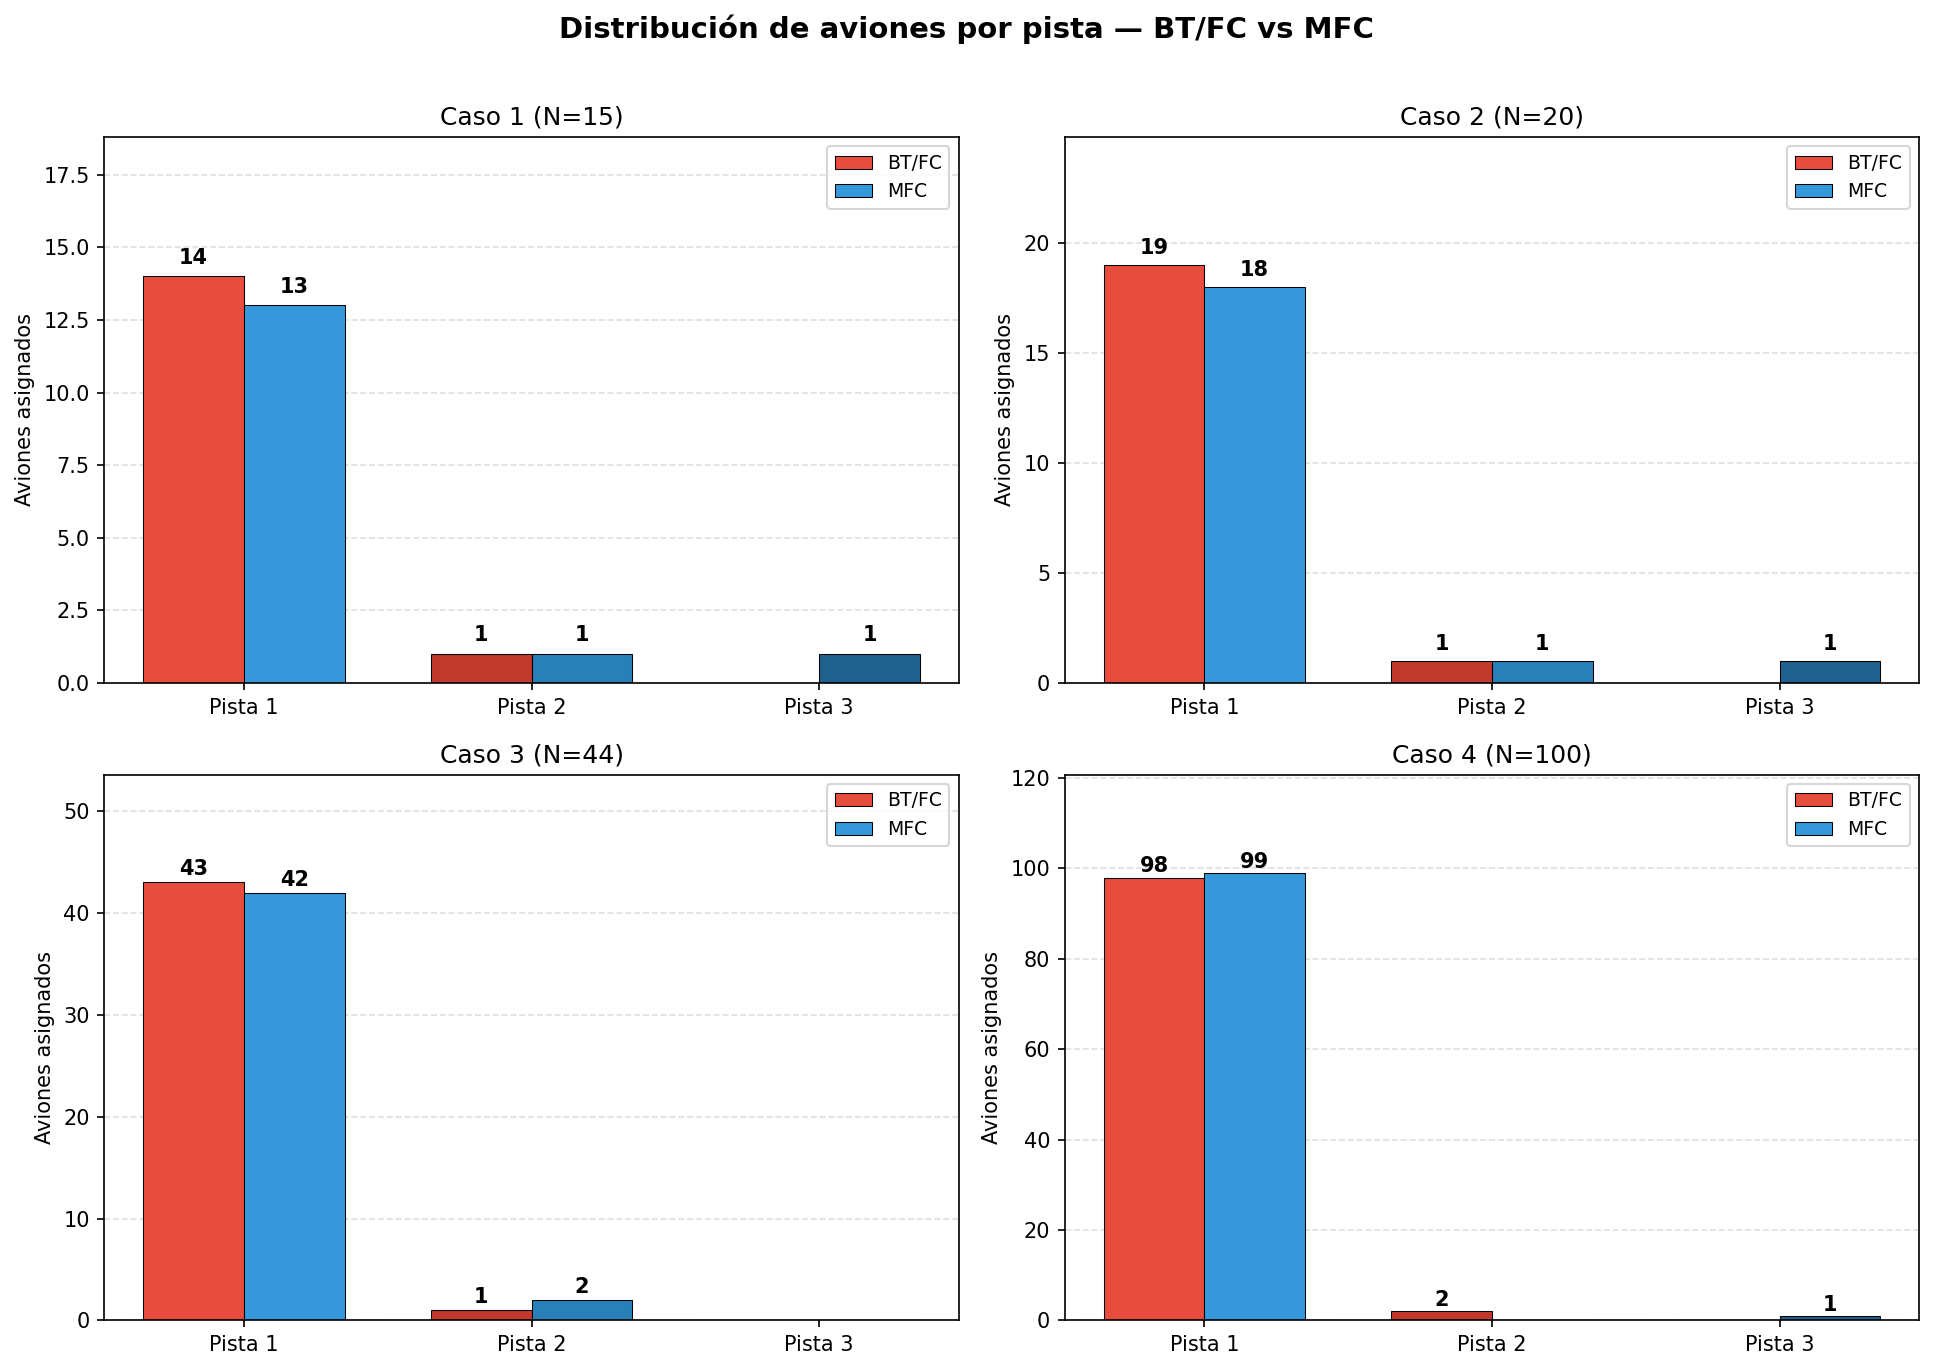
\includegraphics[width=0.95\linewidth]{dist_pistas.png}
    \caption{Distribución de aviones por pista para cada caso y algoritmo (BT/FC vs MFC).}
    \label{graf:dist_pistas}
\end{figure}

\subsection{Convergencia de los casos}

La evolución de la función objetivo en el tiempo demuestra la eficacia de la regla de poda. El gráfico en forma de escalón confirma que el algoritmo realiza caídas rápidas en el costo durante los primeros segundos. Se destaca en el Caso 4, un estancamiento tras encontrar su mejor cota superior, dedicando el resto del límite de tiempo a explorar ramas ineficientes sin lograr reducir el costo.

\begin{figure}[H]
    \centering
    \includegraphics[width=0.7\linewidth]{FOvstiempo.png}
    \caption{Curva de convergencia}
    \label{graf:convergencia}
\end{figure}

% ============================================================
\section*{Declaración de Uso de Inteligencia Artificial}
% ============================================================

Durante el desarrollo del proyecto, se utilizaron herramientas de Inteligencia Artificial como asistencia técnica bajo el rol de ``Guía'', específicamente en los siguientes aspectos:
\begin{itemize}
    \item \textbf{Comprensión y Diseño Heurístico:} Se utilizó la IA para consolidar el entendimiento teórico y la lógica detrás del enfoque \textit{Greedy} (goloso). Esto permitió conceptualizar e implementar correctamente la \textbf{Heurística de Valor} (para priorizar los tiempos de aterrizaje de menor costo) y la \textbf{Heurística de Variable} (para optimizar el orden de asignación de los aviones).
    
    \item \textbf{Sintaxis e Implementación Nativa:} Asistencia en la optimización del código fuente en C++, particularmente en funciones de ordenamiento como \texttt{std::sort} mediante funciones \textit{lambda}, asegurando una ejecución eficiente de las heurísticas diseñadas.
    
    \item \textbf{Benchmarking Computacional:} Apoyo en la estructuración de la lógica de medición de tiempos (librería \texttt{chrono}) para generar el \textit{benchmark} del algoritmo. Esto facilitó el registro preciso de los tiempos de ejecución y la implementación del límite de tiempo de seguridad (\textit{Time Limit}) para las instancias de gran escala.
    
    \item \textbf{Arquitectura de Software:} Orientación para la modularización de la solución en 2 componentes principales: Propagación de las técnicas utilizadas \textit{Minimal Forward Checking} (MFC), \textit{Forward Checking} (FC) y búsqueda recursiva con \textit{backtracking}. Esta organización permitió un código mantenible y facilitó el análisis del comportamiento del árbol de búsqueda.
\end{itemize}

% ============================================================
\section{Análisis Comparativo}
% ============================================================

Para evaluar el rendimiento de los tres algoritmos implementados, se ejecutaron experimentos sobre las cuatro instancias del problema utilizando un límite de tiempo de 15 segundos y 3 pistas disponibles. Los resultados se presentan en las Tablas~\ref{tabla:nodos} y~\ref{tabla:costos}.

\subsection{Nodos Explorados}

\begin{table}[H]
\centering
\renewcommand{\arraystretch}{1.2}
\begin{tabular}{|c|c|c|c|c|}
\hline
\textbf{Instancia} & \textbf{$N$} & \textbf{BT} & \textbf{FC} & \textbf{MFC} \\
\hline
Caso 1 & 15  & 645.810.000 & 270.860.000 & 155.576.625 \\
Caso 2 & 20  & 478.050.000 & 215.640.000 & 147.967.700 \\
Caso 3 & 44  & 170.630.000 & 120.410.000 & 142.458.357 \\
Caso 4 & 100 & 108.390.000 &  88.770.000 & 123.036.613 \\
\hline
\end{tabular}
\caption{Nodos explorados en 15 segundos por algoritmo (3 pistas, con heurística de variable).}
\label{tabla:nodos}
\end{table}

\begin{figure}[H]
    \centering
    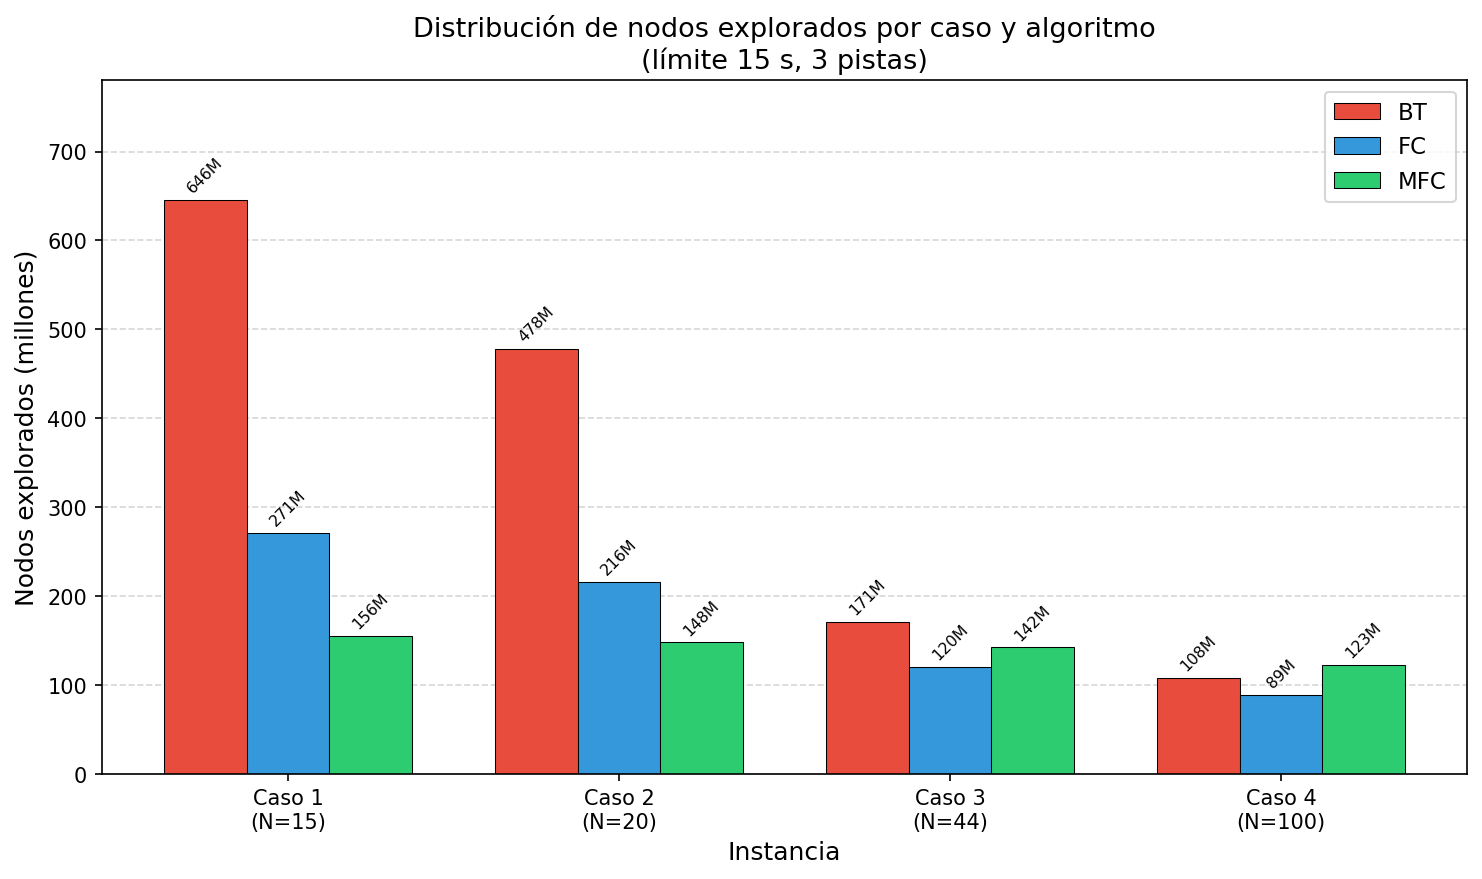
\includegraphics[width=0.85\linewidth]{nodos_por_caso.png}
    \caption{Distribución de nodos explorados por caso y algoritmo (límite 15 s, 3 pistas).}
    \label{graf:nodos_casos}
\end{figure}

\subsection{Costo Mínimo Encontrado}

\begin{table}[H]
\centering
\renewcommand{\arraystretch}{1.2}
\begin{tabular}{|c|c|c|c|c|}
\hline
\textbf{Instancia} & \textbf{$N$} & \textbf{BT} & \textbf{FC} & \textbf{MFC} \\
\hline
Caso 1 & 15  & \$1.860  & \$1.860  & \$3.550  \\
Caso 2 & 20  & \$6.410  & \$6.410  & \$9.140  \\
Caso 3 & 44  & \$3.644  & \$3.644  & \$3.954  \\
Caso 4 & 100 & \$18.794 & \$18.794 & \$37.644 \\
\hline
\end{tabular}
\caption{Costo mínimo encontrado dentro del límite de tiempo (3 pistas, con heurística de variable).}
\label{tabla:costos}
\end{table}

\subsection{Interpretación de Resultados}

\textbf{Comparación BT vs FC.} El FC explora entre un 55\% y un 58\% menos nodos que el BT en todos los casos, encontrando el mismo costo. Esto tiene sentido: el FC elimina valores del dominio de los aviones futuros después de cada asignación, detectando ramas sin salida antes de llegar a ellas. El BT no hace esto, por lo que visita más nodos antes de detectar una infactibilidad. Como ninguno de los dos considera el costo al explorar, ambos terminan encontrando la misma solución dentro del límite de tiempo.

\textbf{Comparación FC vs MFC.} Acá aparece un resultado interesante. En los casos 1, 2 y 3, el MFC explora menos nodos que el FC, pero igual encuentra peores costos. En el caso 4, el MFC explora incluso más nodos que el FC.

Para entender esto, hay que ver la diferencia entre cómo poda cada algoritmo. El FC elimina tiempos individuales del dominio de cada avión futuro: si el tiempo $T'$ viola la separación con el avión recién asignado, $T'$ se borra del dominio. Es una poda detallada, tiempo a tiempo. El MFC en cambio solo actualiza el tiempo mínimo posible (\texttt{E\_dinamico}) de cada avión futuro en esa pista. Solo poda cuando ese mínimo supera el tiempo máximo $L$ en todas las pistas disponibles, lo que se llama \textit{wipe-out}. Es una poda más gruesa.

En los casos 1 a 3, las restricciones de separación son suficientemente ajustadas para que el MFC genere wipe-outs frecuentes, podando ramas enteras antes de expandirlas. Por eso explora menos nodos que el FC. En el caso 4, con 100 aviones y ventanas de tiempo más amplias, los wipe-outs ocurren con menos frecuencia. El MFC propaga sin podar mucho, y además su dominio por nodo queda menos reducido que el del FC. Resultado: más nodos explorados que el FC, más tiempo gastado por nodo en propagación, y en consecuencia menos cobertura del espacio de soluciones dentro del límite de tiempo.

En todos los casos, el MFC encuentra peores costos que BT y FC porque la propagación de restricciones solo sirve para detectar infactibilidad, no para mejorar la calidad de la solución. Sin poda por costo, el MFC cubre menos espacio de búsqueda por segundo y encuentra soluciones de peor calidad.

% ============================================================
\section{Conclusión}
% ============================================================

Este trabajo presentó el diseño e implementación de tres algoritmos exactos para el Problema de Aterrizaje de Aeronaves (ALP) modelado como un CSP de optimización: Backtracking cronológico, Forward Checking y Minimal Forward Checking.

Los experimentos muestran que propagar más restricciones no garantiza encontrar mejores soluciones dentro de un tiempo fijo. El FC explora menos nodos que el BT eliminando tiempos incompatibles de los dominios futuros, y encuentra los mismos costos. El MFC reduce aún más los nodos en instancias pequeñas gracias a los wipe-outs, pero en instancias grandes su poda gruesa es menos efectiva que la poda fina del FC, y su mayor costo por nodo lo deja con menos cobertura del espacio de búsqueda. En todos los casos, al no tener poda por costo, el MFC encuentra peores soluciones que BT y FC dentro del tiempo límite.

El resultado más importante es que la propagación de restricciones del MFC es una herramienta de factibilidad, no de calidad. Su utilidad real aparece cuando se combina con poda por costo, donde detectar infactibilidades temprano ahorra calcular cotas innecesarias. Sola, solo agrega costo computacional.

Ninguno de los tres algoritmos resuelve de forma óptima la instancia de 100 aviones, lo que evidencia la explosión combinatoria del ALP a gran escala. Para instancias de esta magnitud se requieren técnicas complementarias como metaheurísticas o métodos de descomposición.

% ============================================================
\section{Bibliografía}
% ============================================================

\end{document}
